\section{自适应请求 Scheduler}
\label{sec:scheduling}

尽管理论分析显示了较好的结果，但负载不均会降低硬件利用率；在该场景中，我们需要同时考虑两个维度的均衡：（1）NIC 流量，以及（2）GPU 利用率均衡。
我们将调度划分为两个层次：inter-engine scheduling 负责将请求分配给一个（PE, DE）pair，并为每个请求选择读取路径（PE 或 DE）；intra-engine scheduling 则决定每个 forward batch 中包含哪些请求用于计算。

\subsection{Engine 间调度}

我们将 engine 组织成 group，以降低 scheduler 压力。
只有 engine rank $0$（称为 \emph{Leader Engine}）与 scheduler 交互。
一个 group 中的所有 engine 要么全是 PE，要么全是 DE。
同一节点上的所有 engine 保证属于同一 group。
同一 group 中的所有 engine 会定期一起主动 fetch 任务。
在 fetch 新请求时，每个 engine $e$ 上报：（1）$seq_e$，即已分配给它但尚未完成的请求数量；（2）这些 $seq_e$ 个请求上的总 token 数 $tok_e$；（3）engine $e$ 所属节点 $n(e)$ 的磁盘读取队列长度 $read\_q_{n(e)}$。
GPU 负载、磁盘读取负载和网络负载都与 token 数强相关。因此，我们使用 token 数作为代理指标，并目标是在 engine 之间均衡该指标。

\begin{figure}[t!]
  \centering
  % \hspace*{-0.85cm}
  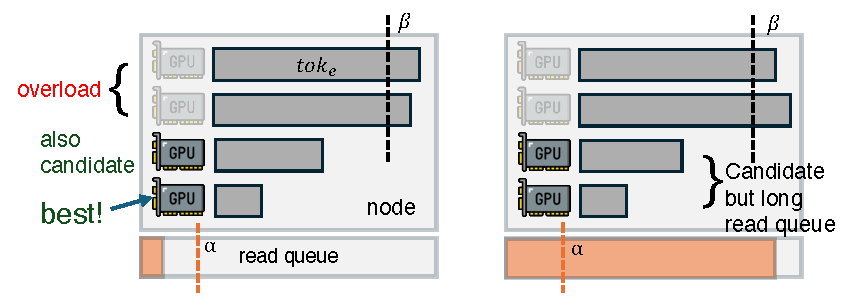
\includegraphics[width=\linewidth]{figures/intersched.pdf}
  \vspace{-0.2in}
  \caption{\normalfont Inter-Engine PE Scheduling 示意图。八块 GPU 都位于同一个 PE engine group 中，scheduler 会选择最优 PE。}
  \vspace{-0.2in}
  \label{fig:intersched}
\end{figure}

\parabf{PE 调度。} 所有到达 scheduler 的请求进入等待队列，并按 FIFO 顺序调度。当某个 PE group 发起 fetch request 时，调度算法被调用。
Inter-engine 调度过程示意见 \autoref{fig:intersched}。
我们定义两个常数：短读取队列阈值 $\alpha$，以及未完成 token 上限 $\beta$（以 token 为单位）。
所有 engine 被划分为三类：
(1) 过载 engine，满足 $tok_e > \beta$；
(2) 位于短磁盘读取队列节点上的 engine，满足 $read\_q_{n(e)} \leq \alpha$ 且 $tok_e \leq \beta$；
(3) 位于较长磁盘读取队列节点上的 engine，满足 $read\_q_{n(e)} > \alpha$ 且 $tok_e \leq \beta$。
我们不会向过载 engine 分配新请求。
第二类 engine 优先级高于第三类，因为它们所在节点的磁盘读取队列更短；如果后续请求不足，容易导致存储 NIC 利用不足。

若第二类非空，我们将当前请求分配给第二类中 $tok_e$ 最小的 PE；否则若第三类非空，则分配给第三类中 $tok_e$ 最小的 PE。
分配后，我们更新被选中 PE 的 $tok_e$，然后处理等待队列中的下一个请求。
如果两类都为空，则终止本次 fetch request，并将已经分配的请求返回给 Leader Engine。



\begin{algorithm}[t]
\caption{\normalfont Inter-PE 调度算法}
\label{alg:pe-scheduling}
\SetAlgoLined
\KwData{等待队列 $Q$，PE group $G_{PE}$，每个 engine $e$ 上报的负载指标 $(read\_q_{n(e)}, tok_e)$，其中 $n(e)$ 表示 engine $e$ 所属节点，常数 $\alpha$ 和 $\beta$}
\KwResult{分配给 PE 的请求}
\BlankLine
每个 engine $e$ 上报 $(read\_q_{n(e)}, tok_e)$\;
将所有 PE 划分为三类：\;
\Indp $C_1 \leftarrow \{e \in G_{PE} : tok_e > \beta\}$\;
$C_2 \leftarrow \{e \in G_{PE} : read\_q_{n(e)} \leq \alpha \wedge tok_e \leq \beta\}$\;
$C_3 \leftarrow \{e \in G_{PE} : read\_q_{n(e)} > \alpha \wedge tok_e \leq \beta\}$\;
\Indm
\While{$Q$ is not empty}{
    $r \leftarrow$ $Q$ 的队首请求\;
    \eIf{$C_2 \neq \emptyset$}{
        $pe^* \leftarrow \arg\min_{e \in C_2} tok_e$\;
    }{
        \eIf{$C_3 \neq \emptyset$}{
            $pe^* \leftarrow \arg\min_{e \in C_3} tok_e$\;
        }{
            终止本次 fetch request\;
            将已分配请求返回给 Leader Engine\;
            \textbf{break}\;
        }
    }
    将请求 $r$ 分配给 PE $pe^*$\;
    更新 $tok_{pe^*} \leftarrow tok_{pe^*} + \text{tokens}(r)$\;
    从 $Q$ 中移除 $r$\;
}
\end{algorithm}


\parabf{DE 调度阶段 1：跨 group。}
DE 调度分为两层，且不保持全局 FIFO。系统有一个全局等待队列，以及每个 DE engine group 的私有队列。新到达请求首先进入全局队列。当某个 DE group fetch 时，\emph{group-level} 调度会从全局队列取出请求，并将每个请求分配给总 $tok_e$（该 group 内所有 engine 之和）最小的 group；这会在 group 之间均衡 token 数，从而均衡 NIC 和 GPU 负载。

\parabf{DE 调度阶段 2：group 内。}
然后，我们计算该 group 中所有 DE 的剩余 HBM 总和，并从私有队列队首开始遍历，假设没有 HBM 碎片，计算有多少请求可以被调度。这些请求形成集合 $R$。
它是可调度请求集合的上界。
随后，我们计算一个高 token 阈值 $Z = 1.05 \times (\sum_{r\in R} {len_r} + \sum_{e\in E} {tok_e}) / |E|$。

接下来，我们尝试弹出私有队列队首请求，并将其调度到某个 DE。
在剩余 HBM 足够容纳该请求的 DE 中，我们划分两类：（1）高 token DE，满足 $tok_e + \text{len}(r) > Z$；（2）其余 DE。我们优先选择第（2）类，以保持 token 数均衡；第（1）类 DE 已经具有较高 GPU 和 NIC 压力。在第（2）类内部，我们选择 $seq_e$ 最小的 DE 来均衡请求数量；如果第（2）类为空，则选择第（1）类中 $tok_e$ 最小的 DE，以降低 HBM 耗尽和抢占风险。如果没有 DE 具备足够 HBM，则本次 fetch 结束，并返回已分配请求。

\parabf{KV-Cache 读取任务调度。} 
在为请求选定 PE 和 DE 后，我们选择读取队列更短的一侧执行读取。将请求拆成两部分并从两侧同时读取可能更好，我们将其留作未来工作。

\subsection{Engine 内调度}

只有 PE 需要 intra-engine scheduling，因为 DE 总是将所有请求放入 forward batch。
Intra-engine 调度过程示意见 \autoref{fig:intrasched}。
Data parallelism 被广泛用于 attention 层，尤其是 MLA 模型。
在这种并行配置下，每块 GPU 服务不同请求集合。
这可能导致所有 GPU 之间工作负载不均，而它们必须在 attention 阶段之后同步并一起进入 FFN 阶段，从而造成 GPU bubble 等待其他 peer。
因此，我们需要确保它们具有相近的 attention 层执行时间，以最小化等待 bubble。


\begin{figure}[t!]
  \centering
  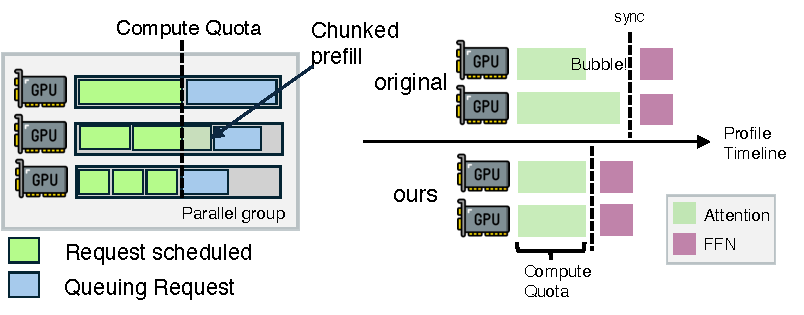
\includegraphics[width=\linewidth]{figures/intrasched.pdf}
  \caption{\normalfont Intra-Engine 调度。左：基于 compute quota 的 batch 选择。右：应用 compute quota 前后的 GPU timeline。}
  \label{fig:intrasched}
\end{figure}

\parabf{层时间估计。} 我们使用 FIFO packing 来决定一个 forward batch 中包含多少请求。
Forward batch 中的每个请求由一对 $(cached, bsz)$ 描述，其中 $cached$ 是 KV-Cache 已可用的 token 数（来自存储命中或先前 forward pass），$bsz$ 是本次 forward batch 中需要计算 KV-Cache 的 token 数。
基于这些 pair，我们计算 attention 层的理论总计算量，并估计其执行时间。
理论计算量与 wall-clock 时间之间的关系取决于硬件和并行配置，可以像已有工作~\cite{SOSP25:PrefillOnly} 和~\cite{OSDI24:SarathiServe} 一样，通过预先 profiling 拟合得到。

\parabf{算法。} 只要预测的 attention 层执行时间不超过预定义上限，我们就按 FIFO 顺序不断加入请求。该上限称为\emph{compute quota}。
如果加入某个请求会超过该上限，我们会对 $bsz$ 执行二分搜索，找到一个更小的 $bsz'$ 来适配剩余 compute quota，并对该请求执行 chunked prefill。
